In this section, we discuss a representative running examples with
challenges of analyzing the symbolic
\emph{reachability-bound} on
every control location and illustrate our key technique novelties, the \emph{path reachability-bound} and the \emph{loop reachability-bound}.
This example is adopted from the example in~\cite{GulwaniZ10}, which
is a skeleton code from the .Net base-class library.

% \paragraph{Challenges.}
%\begin{example}
 % [The Running Example with Nested Loop in One Path]
%  \label{ex:relatedNestedWhileOdd-overview}
{ \small
% \vspace{-0.2cm}
\begin{figure}
\centering
\begin{subfigure}{.4\textwidth}
\begin{centering}
{\small
$
\begin{array}{l}
  \kw{nestedOdd}(n, m) \triangleq \\
  \clabel{ \assign{i}{n} }^{0} ; \\
      L_1: \ewhile ~ \clabel{i > 0}^{1} ~ \edo ~ \\
      \quad \big(
        \eif(\clabel{i \% 2 \neq 0 }^{2},
        \clabel{\assign{k}{i - m}}^{3};\\
        \quad L_4: \ewhile ~ \clabel{k > 0}^{4} \edo \\
        \quad ( \clabel{\assign{k}{k - 1}}^{5} );\\
        \quad \clabel{\assign{i}{k + m}}^{6};
        \clabel{\assign{i}{i - 1}}^{7}, \\
        \quad \clabel{\assign{i}{i - 3}}^{8})
        \big)
  \end{array}
$
}
\vspace{-0.3cm}
\caption{}
\end{centering}
\end{subfigure}
\begin{subfigure}{.52\textwidth}
\begin{centering}
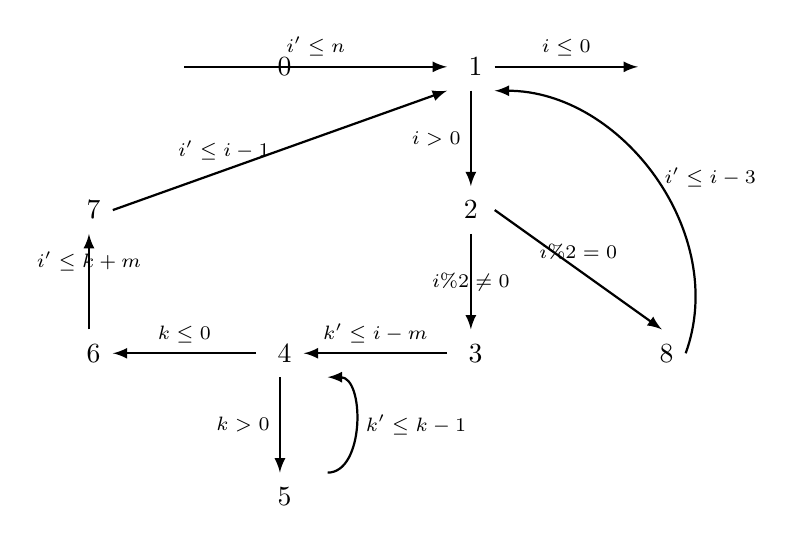
\begin{tikzpicture}[scale=\textwidth/20cm,samples=200]
\draw[] (-4, 10) circle (0pt) node{{ $0$}};
\draw[] (0, 10) circle (0pt) node{{ $1$}};
\draw[] (0, 7) circle (0pt) node{\textbf{$2$}};
\draw[] (0, 4) circle (0pt) node{{ $3$}};
\draw[] (-4, 4) circle (0pt) node{{ $4$}};
\draw[] (-8, 4) circle (0pt) node{{ $6$}};
\draw[] (-4, 1) circle (0pt) node{{ $5$}};
\draw[] (4, 4) circle (0pt) node{{ $8$}};
\draw[] (-8, 7) circle (0pt) node{{ $7$}};
% Counter Variables
\draw[] (4.5, 10) circle (0pt) node {\textbf{$\lex$}};
% \draw[] (6, 4) circle (0pt) node {{ $ex$}};
%
% Control Flow Edges:
\draw[ thick, -latex] (-6, 10)    -- node [above]{\scriptsize $i' \leq n$}(-0.5, 10);
\draw[ thick, -latex] (0, 9.5)    -- node [left] {\scriptsize $i > 0$} (0, 7.5) ;
\draw[ thick, -latex] (0.5, 7)    -- node [above] {\scriptsize $ i \% 2 = 0 $}  (4, 4.5);
\draw[ thick, -latex] (4.5, 4)    to  [out=70,in=0]   node [right] {\scriptsize $i' \leq i - 3$ }(0.5, 9.5);
\draw[ thick, -latex]  (0, 6.5)   -- node  {\scriptsize $i \% 2 \neq 0$}  (0, 4.5) ;
\draw[ thick, -latex]  (-0.5, 4)  -- node [above] {\scriptsize $k' \leq i - m$ }  (-3.5, 4) ;
\draw[ thick, -latex]  (-4.5, 4)  -- node [above] {\scriptsize $k \leq 0$ }  (-7.5, 4);
\draw[ thick, -latex] (0.5, 10)   -- node [above] {\scriptsize $i \leq 0$}  (3.5, 10);
\draw[ thick, -latex] (-4, 3.5)   -- node [left] {\scriptsize $k > 0$}  (-4, 1.5);
\draw[ thick, -latex] (-3, 1.5)   to  [out=0,in=0] node [right] {\scriptsize $k' \leq k- 1$}  (-3, 3.5);
\draw[ thick, -latex] (-8, 4.5)   --  node [above] {\scriptsize $i' \leq k + m$ }(-8, 6.5);
\draw[ thick, -latex] (-7.5, 7)  --  node [left] {\scriptsize $i' \leq i - 1$ }(-0.5, 9.5);
% \draw[ thick, -latex] (6, 6.5)  -- node [right] {$\top$} (6, 4.5) ;
\end{tikzpicture}
\vspace{-0.5cm}
\caption{}
\end{centering}
\end{subfigure}
\begin{subfigure}{.9\textwidth}    
\begin{centering}
{\small
$\tpath_0 = (0 \to 1)$
\quad
$\tpath_1 = (1 \to 2 \to 3 \to 4)$
\quad
$\tpath_2 = (4 \to 6 \to 7 \to 1)$
\quad
$\tpath_3 = (4 \to 5 \to 4)$
\quad
$\tpath_4 = (1 \to 2 \to 8 \to 1)$
\quad
$\tpath_5 = (1 \to \lex)$
}
\vspace{-0.3cm}
\caption{}
\end{centering}
\end{subfigure}
% \vspace{-0.5cm}
\begin{subfigure}{.8\textwidth}    
  \begin{centering}
  $
  \tpath_0 ; \rpchoose{ 1: \rprepeat(\tpath_1; 4:\rprepeat(\tpath_3); \tpath_2; \tpath_4), 
  1: \rprepeat(\tpath_4; \tpath_1; 4:\rprepeat(\tpath_3); \tpath_2) }; \tpath_5
  $
  % \vspace{-0.5cm}
  \caption{}
  \end{centering}
  \end{subfigure}
\caption{
(a) Running example: program with a loop with two  paths and a nested loop in one of them,
(b) the corresponding \emph{abstract transition graph}, $\absG(\kw{nestedOdd}(n, m))$,
(c) all the simple transition paths on this program,
(d) the refined program.}
% \vspace{-0.75cm}      
\label{fig:relatedNestedWhileOdd-overview}
\end{figure}
}
%  \footnotetext{In the transition path, $(l_0 \to \cdots \to l_n)$, the constraints are omitted for concise.}
%
%  \end{example}    

% \todo{Shorten}
% \begin{itemize}
%   \item 
\textbf{Challenge I}
  In this example, given $n \geq m \geq 0$,
the expected \emph{reachability-bound}s for locations $3, 6, 7$ and $8$ are all $\lfloor\frac{m}{4}\rfloor$,
%  for $8$ is $\lfloor\frac{m}{4}\rfloor + 1$,
for location $2$ is $\lfloor\frac{m}{2}\rfloor$ and $\lfloor\frac{m}{2}\rfloor + 1$ for location $1$.
\highlight{Notice here, though within the same loop $L_1$, the bounds for different locations are different.}
The amortized analysis methodology (inlcuding Loopus in~\cite{SinnZV17}, KoAT~\cite{BrockschmidtEFFG14,FalkeKS12,FalkeKS11}, C4B~\cite{CarbonneauxHS15}) ignores path sensitivity and approximate the bound $n$ as the bound for loop $L_1$. 
And the path-refinement based method (\cite{GulwaniZ10} and \cite{GulwaniJK09} and CoFloCo~\cite{Montoya17,Flores-Montoya16,Flores-MontoyaH14}) only give the same bound for all the locations within the loop $L_1$. 
% The SPEEDi in~\cite{GulwaniZ10}
% gives the same \emph{reachability-bound}, $n + \lfloor\frac{n}{m}\rfloor$ for all the locations within the loop $L_2$. Though is tight w.r.t. $L_1$'s iteration times but not \emph{reachability-bound} for different locations.
% \cite{GulwaniJK09}, the Loopus in~\cite{SinnZV17}, KoAT~\cite{BrockschmidtEFFG14,FalkeKS12,FalkeKS11}, C4B~\cite{CarbonneauxHS15} and CoFloCo~\cite{Montoya17,Flores-Montoya16,Flores-MontoyaH14} also can only compute the bound on the loop iteration but not reachability-bound on each location path-sensitively.
Though we can reuse their estimated loop bounds as the \emph{reachability-bound} for location $1$ and $2$,
the \emph{reachability-bounds} for control locations $3, 6, 7$ and $8$ are still unclear.
%
This motivates our first key novelty -- the \emph{path reachability-bound} $\inoutB(\rprog, \tpath)$ for a loop free and interleaving free path $\tpath$.
It bounds the evaluation times of each path over a path-refined program.
% \item 

\textbf{Challenge II} The second challenge occurs in the nested loop.
In line 6, $i$ is reset by $k + m$ and $k$ is reset by $i - m$ at line 3. So the
loop $L_4$ is only executed in the first iteration of while loop $L_1$.
% \\
% The while loop $L_1$ at line 3 is executed only in 
% the first $m - N$ iterations of the 
% $L_1$ because $j$ is reset by $i$ in line 2.
% \\
So the total iterations of all the two loops are
$n - m + \lfloor\frac{m}{2}\rfloor + 1$,
and the precise \emph{reachability-bound} for location $5$ inside the $L_4$ is $m$.
% for locations $4, 5$ and $8$ between the $L_3$ and $L_6$ are $(n-N) \times (m - N)$,
% and $n - N$ for locations $2$ and $9$.
% \\
\highlight{Notice here the \emph{reachability-bounds} for the locations inside the loop $L_4$ is 
the same as its innermost loop iteration bound.
% , as well as our \emph{path reachability-bound}.
However, for the locations between $L_1$ and $L_4$,
the \emph{reachability-bounds} are the multiplication of the inner and outer loop iteration bounds.}
% \\
% To the best of our knowledge, the loop bound analysis method in \cite{GulwaniJK09} can only give a loose bound $n + (m \times n) + N$ for the entire loop complexity, and 
% the DC-based algorithm in \cite{SinnZV17} is able to
% compute a better but still loose bound, $n + m^2 - m \times N$ on total iteration times.
Again, existing approach either ignores the path sensitivity (in the ) or computes the same bound for all the locations in a loop.
None of them can give the precise \emph{reachability-bound}s for different locations in the loop,
which is non-trivial to compute even though knowing the loop bound.
% especially for the locations similar to $7$ in $\kw{threeNestedWhile}$.

\highlight{
This motivates us to consider our second novel quantity --
the numbers of iterations of the outside loop $L_1$ such that,
during these iterations, the loop $L_4$ is ``entered''. 
We refer this quantity as the \emph{loop reachability} of the loop $L_4$ w.r.t the outer loop $L_1$.
% of the location within loop $L_6$ w.r.t the loops $L_3$ and $L_1$.
By multiplying the \emph{path reachability-bound} of $\tpath_3$ within $L_4$,
with its \emph{loop reachability-bound} w.r.t $L_1$, we can obtain an accurate
\emph{reachability-bound} for location $5$.
This quantity isn't considered or computed in any of the previous works.
Paper~\cite{GulwaniJK09} consider a similar quantity, the \emph{Progress Invariant}. While this quantity is a bound on the iteration times of inner loop $L_4$ w.r.t. one iteration of $L_1$, which is $m$. Then they still over-approximate the bound for locations inside $L_4$ as $m \times (n - m)$ by multiplication.
% In the line of methods based on path refinement and loop summarization, the \emph{Progress Invariant} method in~\cite{GulwaniJK09} is only able to compute
% the
% bound on iteration numbers
% of the inner loop $L_4$ in one iteration of $L_1$, which is $m$.
% So they have to over-approximate the reachability-bound for locations inside $L_4$ with the
% overall program complexity by multiplication as $m \times (n - m)$.
% In the line of the \emph{amortized complexity analysis} through ranking function, the LoopusJAR~\cite{SinnZV17}
% is only able to
% compute the combined loop bound and the local bound of each loop
% separately as well.
% We are still unable to know the precise \emph{reachability-bound} for the locations in the innermost loop.
}

% \end{itemize}
With the two key novelties, our algorithm computes the reachability-bound for this example through the following steps.


\textbf{Step 1: }
The Section~\ref{sec:progabs} first 
computes the \emph{Abstract Transition Graph} as in Figure~\ref{fig:relatedNestedWhileOdd-overview}(b).
Each edge $l \xrightarrow{dc} l'$ is an abstract transition $\absevent = (l, dc, l')$ annotated with a constraint $dc$ corresponding to the command of label $l$.

% \textbf{Step 2: Program Refinement}
\textbf{Step 2: }
The second step in Section~\ref{sec:refine}
computes the \emph{Refined Program}, $\rprog$ for a program $c$ based on 
its abstraction transition graph and transforms the multiple-paths loops
into multiple loops where
the interleaving of paths is explicit as in bottom part of Figure~\ref{fig:relatedNestedWhileOdd-overview}(c).
It has two interleaving patterns in the loop $L_1$.
%  denoted as $\rprog_1^1$ and $\rprog_1^2$.

% \textbf{Step 3: Ranking Function Estimation}
\textbf{Step 3: }
In the meanwhile, Section~\ref{sec:rank} computes the \emph{Ranking Function}, $\locbound(\absevent, c)$ 
for every edge $\absevent$ 
and estimates an upper bound invariant for each.

% \textbf{Step 4: Path-sensitive Reachability-bound Computation.}
\textbf{Step 4: }
% The \emph{path-sensitive reachability-bound} 
The algorithm computes the \emph{Reachability-bound}, $\psRB(l, c)$ for every program point $l$ using the $\rprog$ and the upper bound invariant of the $\locbound(\absevent, c)$ where $\absevent = (l,dc,l')$.
It requires to compute our two novel quantities, the \emph{Path Reachability-bound}, $\inoutB(\rprog, \tpath, c)$ and the \emph{Loop Reachability-bound}, $\lpchB(l: \rprog, \tpath, c)$.
Section~\ref{sec:psrb} introduces this algorithm and the following sections describe the computations. 
The soundness of each algorithm is in the Appendices and the input $c$ will be omitted if the context is clear.

In the first interleaving pattern, $\rprog_1^1 = 1: \rprepeat(\tpath_1; 4:\rprepeat(\tpath_3); \tpath_2; \tpath_4)$ in Figure~\ref{fig:relatedNestedWhileOdd-overview},
we first compute $\outinB(4:\rprepeat(\tpath_3), \tpath_3) = n - m$
 for $\tpath_3$ in its innermost loop $L_4$ as a local \emph{path reachability-bound} by Section~\ref{sec:pathlocalrb}.
Then we compute $\lpchB(\rprog_1^1, \tpath_3) = 1$ w.r.t. its outer loop $L_1$ in Section~\ref{sec:looprb}. In the second interleaving pattern, we compute $\outinB(4:\rprepeat(\tpath_3), \tpath) = n - m - 3$ and the same for $\lpchB$.
So Section~\ref{sec:pathrb} computes $\inoutB(\rprog, \tpath_3) = \max\{ 1 \times (n - m), 1 \times (n - m - 3) \} = n - m$ globally.

Then for every program point $l$, we sum up all the $\inoutB(\rprog, \tpath)$ over $\tpath$ that contains $l$ and get $\psRB(l, c)$.
Since point $5$ only shows up on $\tpath_3$, we compute \highlight{$\psRB(5, c) = n - m$}.
The points $0$ and $\lex$ are not in any loop, so $\psRB(0) = \psRB(\lex) = 1$,
The points $3, 6, 7$ and $8$ which only show up once on $\tpath_2$ and $\tpath_4$ are all equal to $\lfloor\frac{m}{4}\rfloor$, which are same as their $\inoutB$.
For the loop headers $1$ and $4$, we only sum up the $\inoutB(\rprog, \tpath)$ where they show up as start-point of the $\tpath$.
So $\psRB(4) =  \lfloor\frac{m}{4}\rfloor + n - m + 1$ and $\psRB(1) = 2 \times \lfloor\frac{m}{4}\rfloor + 1$ all as expected.
% For the other points in different branches and loop, we compute
% $\psRB(1) =2 \times \lfloor\frac{m}{4}\rfloor + 1$,
% $\psRB(2) =2 \times \lfloor\frac{m}{4}\rfloor $, 
% $\psRB(3) = \psRB(6) = \psRB(7)  = \psRB(8) = \lfloor\frac{m}{4}\rfloor $,
% \highlight{$\psRB(5) = \lfloor\frac{m}{4}\rfloor \times 1$},
% and $\psRB(4) =  \lfloor\frac{m}{4}\rfloor + n - m + 1$ as expected.


%     % Our static program analysis algorithm computes 
% % a \emph{reachability-bound} for every program point $l$ in a program $c$ in a path sensitive manner.
% % The main steps of this algorithm and the organization the following sections are summarized as follows.
% \begin{enumerate}
%     \item  The Section~\ref{sec:progabs} first 
%     computes the \emph{Abstract Transition Graph}, $\absG(\kw{nestedOdd})$ as in Figure~\ref{fig:relatedNestedWhileOdd-overview}(b).
%     Each edge $l \xrightarrow{dc} l'$ is an abstract transition with annotated with a constraint corresponding to the command of label $l$.
%     \item The second step in Section~\ref{sec:refine}
%     computes the \emph{Refined Program}, $\rprog$ for a program $c$ based on 
%     its abstraction transition graph and transforms the multiple-paths loops
%     into multiple loops where
%     the interleaving of paths is explicit as in bottom part of Figure~\ref{fig:relatedNestedWhileOdd-overview}(c).
%     \item In the same time of refining the program, we also compute the \emph{Ranking Function} in Section~\ref{sec:rank}
%     for every edge 
%     and estimate the upper bound invariant w.r.t, the input variables on every ranking function's maximum value.
%     \item The \emph{path-sensitive reachability-bound} algorithm computes the \emph{reachability-bound}, $\psRB(l, c)$ for every program point.
%     It relies on the \emph{Refined Program} and the upper bound invariant of the \emph{Ranking Function} computed previously.
%     It requires to compute our two novel quantities, the \emph{Path Reachability-bound}, $\outinB(\rprog, \tpath)$ and the \emph{Loop Reachability-bound}, $\lpchB(l: \rprog, \tpath)$.

%     For the transition path $\tpath_3 = 4 \to 5 \to 4$ in the first interleaving pattern where $\rprog_1^1 = 1: \rprepeat(\tpath_1; 4:\rprepeat(\tpath_3); \tpath_2; \tpath_4)$,
%     we compute $\outinB(4:\rprepeat(\tpath_3), \tpath) = m$ w.r.t its innermost loop $L_4$ as a local \emph{Path Reachability-bound} in Section~\ref{sec:pathlocalrb}
%     We also compute $\lpchB(\rprog_1^1, \tpath) = 1$ w.r.t. its outer loop $L_1$ in Section~\ref{def:looprb},
%     and Section~\ref{sec:pathrb} computes $\tpath_3$'s global \emph{Path Reachability-bound} $\inoutB(\rprog, \tpath) = m$.

%     By summing up all the \emph{path reachability-bounds}, $\inoutB(\rprog, \tpath)$ over the $\tpath$ which contains the program point $l$, we compute the \emph{Reachability-bound}, $\psRB(l, c)$ for every program point $l \in \lvar(c)$.
%     For the points $0$ and $\lex$ which aren't in any loop, we compute $\psRB(0) = \psRB(\lex) = 1$,
%     For the other points in different branches and loop, we compute $\psRB(1) =2 \times \lfloor\frac{m}{4}\rfloor + 1$,
%     $\psRB(2) =2 \times \lfloor\frac{m}{4}\rfloor $, 
%     $\psRB(3) = \psRB(6) = \psRB(7)  = \psRB(8) = \lfloor\frac{m}{4}\rfloor $,
%     \highlight{$\psRB(5) = \lfloor\frac{m}{4}\rfloor \times 1$},
%     and $\psRB(4) =  \lfloor\frac{m}{4}\rfloor + n - m + 1$ as expected.

%     Section~\ref{sec:psrb} introduces this algorithm and the following sections describe the computations. 
%     % To compute the \emph{reachability-bound}  compute the path reachability-bound for 
%     % We compute the $\lpchB(l: \rprog, \tpath)$ for 
%     % \begin{enumerate}
%         % \item Based on the ranking function and its upper bound invariant, we first compute the \emph{Path Local Reachability-bound}, $\outinB(\rprog, \tpath)$ for every \emph{simple transition path} $\tpath$ in Section~\ref{sec:pathlocalrb}. 
%         % This bounds the reaching / visiting times of $\tpath$ when executing program $\rprog$, and $\rprog$ is the closest loop where $\tpath$ is nested.
%         % The local reachability-bound  considers only the execution of $\tpath$'s closest enclosing loop, i.e., $\kw{enclosed}(\tpath)$.
%         % \item Then in Section~\ref{sec:looprb}, we compute the \emph{Loop Reachability-bound}, $\lpchB(l: \rprog, \tpath)$ for every \emph{simple transition path} $\tpath$
%         % w.r.t its nested loop. 
%         % This is the bound on iteration numbers of the outside loop $l$,
%         % such that during these iterations, the nested loop $l' = \kw{enclosed(\tpath)}$ is executed, i.e., reached.
%         % \item The \emph{Path Reachability-bound}, $\inoutB(\rprog, \tpath)$  is a global upper bound on the execution times of a \emph{simple transition path} $\tpath$ computed in Section~\ref{sec:pathrb}.
%         % With the global reachability-bound of every simple transition path, now we can sum up all the \emph{path reachability-bounds}, $\inoutB(\rprog, \tpath)$ over the $\tpath$ which contains the program point $l$, and compute the \emph{Reachability-bound}, $\psRB(l, c)$ for every program point $l \in \lvar(c)$ as in Definition~\ref{def:point_psrb}.
%     % \end{enumerate}
%     \end{enumerate}



% % The second key idea combining two lines of works above is the \emph{loop reachability-bound}, $\lpchB(L:\rprog, \tpath)$.
% % For each transition path $\tpath$ w.r.t each of the loops $L:\rprog$ in which $\tpath$ is nested,
% % $\lpchB(L:\rprog, \tpath)$ bounds the iterations for
% % the outside loop, $L:\rprog$ w.r.t. the innermost loop where $\tpath$ is enclosed,
% % such that during these iterations of $L:\rprog$, the innermost loop is ``entered''. 
% % Then by multiplication and summing over these two bounds where each program control point shows up, we compute each point's the \emph{reachability-bound} path-sensitively.

% \paragraph{The path reachability-bound}, $\inoutB(\rprog, \tpath)$ is our first key novelty.
% It is a bound for a loop free path $\tpath$ within a loop program $\rprog$ bounds the evaluation times of each loop free path instead of the entire multipath loop.
%     { \footnotesize
    \begin{figure}
    \centering
    %
    \begin{subfigure}{.27\textwidth}
        $
        \begin{array}{l}
          \kw{twoPathsWhile}(n, m) \triangleq \\
        \clabel{ \assign{i}{n} }^{0} ;
        \clabel{ \assign{j}{0} }^{1} ; \\
        L_2:    \ewhile ~ \clabel{i > 0}^{2} ~ \edo ~ \\
            \qquad \big(
              \eif(\clabel{j < m}^{3}, \\
              \qquad \ethen  \clabel{\assign{j}{j + 1}}^{4}; \\
              \qquad \qquad \clabel{\assign{i}{i - 1}}^{5},\\
              \qquad \eelse \clabel{\assign{j}{0}}^{6});
              \big)
            \end{array}
            $
\vspace{-0.2cm}
\caption{}
\end{subfigure}
\begin{subfigure}{.71\textwidth}
\begin{subfigure}{.67\textwidth}
\begin{centering}
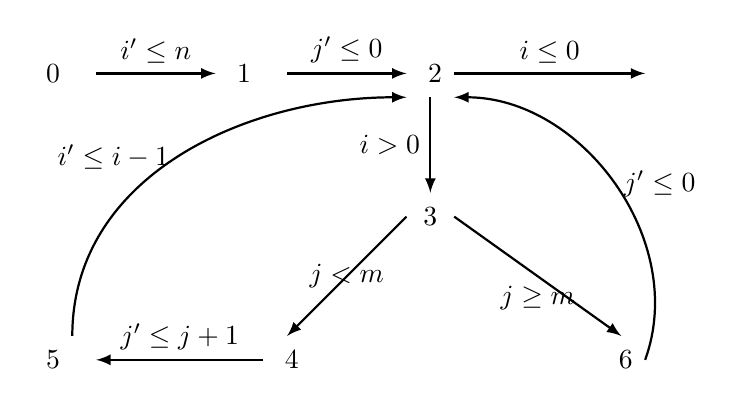
\begin{tikzpicture}[scale=\textwidth/20cm,samples=200]
    \draw[] (-8, 10) circle (0pt) node{{ $0$}};
    \draw[] (-4, 10) circle (0pt) node{{ $1$}};
    \draw[] (0, 10) circle (0pt) node{{ $2$}};
    \draw[] (0, 7) circle (0pt) node{{$3$}};
    \draw[] (-3, 4) circle (0pt) node{{ $4$}};
    \draw[] (-8, 4) circle (0pt) node{{ $5$}};
    \draw[] (4, 4) circle (0pt) node{{ $6$}};
    % Counter Variables
    \draw[] (5, 10) circle (0pt) node {\textbf{$\lex$}};
    %
    % Control Flow Edges:
    \draw[ thick, -latex] (-7, 10)  -- node [above] {$i' \leq n$}(-4.5, 10);
    \draw[ thick, -latex] (-3, 10)  -- node [above] {$j' \leq 0$}(-0.5, 10);
    \draw[ thick, -latex] (0, 9.5)  -- node [left] {$i > 0$} (0, 7.5) ;
    \draw[ thick, -latex] (0.5, 7)  -- node [below] {$ j \geq m $}  (4, 4.5);
    \draw[ thick, -latex] (-7.5, 4.5)  to  [out=90,in=180]  node [left] {$i' \leq i - 1$ }(-0.5, 9.5);
    \draw[ thick, -latex] (4.5, 4)  to  [out=70,in=0]   node [right] {$j' \leq 0 $}(0.5, 9.5);
    \draw[ thick, -latex]  (-0.5, 7) -- node  {$j < m$}  (-3, 4.5) ;
    \draw[ thick, -latex]  (-3.5, 4) -- node [above] {$j' \leq j + 1$}  (-7, 4) ;
    \draw[ thick, -latex] (0.5, 10)  -- node [above] {$i \leq 0$}  (4.5, 10);
  \end{tikzpicture}
        \caption{}
\end{centering}
\end{subfigure}
{\small
\begin{subfigure}{.3\textwidth}
\begin{centering}
        $\tpath_0 = 0 \to 1 \to 2$ \\
        $\tpath_2 = 2 \to 3 \to 6 \to 2$ \\ 
        $\tpath_1 = 2 \to 3 \to 4 \to 5 \to 2$ \\
        $\tpath_3 = 2 \to \lex$
        \caption{}
\end{centering}
\end{subfigure}
}
{\small
\begin{subfigure}{.8\textwidth}
\begin{centering}
    $
    \tpath_0 ; 
    \rpchoose{2: \rprepeat(\rprepeat(\tpath_1); \tpath_2), 
    2: \rprepeat(\tpath_1)}; \tpath_3.
    $
\end{centering}
\end{subfigure}
}
\end{subfigure}
\vspace{-0.2cm}
\caption{
    (a) The two paths loop example,
    (b) the Abstract Transition Graph for $\kw{twoPathsWhile}(n, m)$,
    (c) the Simple Transition Paths of $\kw{twoPathsWhile}(n, m)$.}
    \vspace{-0.5cm}
        \label{fig:whileTwoCounters-overview}
    \end{figure}
    }



% \footnotetext{We use the notation $(l_0 \to \cdots \to l_n)$ to denote a vertices sequence $(l_0, \cdots, l_n)$, and the constraint on each edge in each transition path are omitted for concise.}
% Figure~\ref{fig:whileTwoCounters-overview}(a) shows an example of a two paths loops
% with different \emph{reachability-bounds} on the control locations in different paths.
% This example is adopted from the example in~\cite{GulwaniZ10}, which
% is a skeleton code from the .Net base-class library.
% \\
% In this example, given $n \geq m$,
% the precise \emph{reachability-bound}s for control locations $4$ and $5$ are both $m \times \lfloor\frac{n}{m}\rfloor$,
% for location $2$ and $3$ are $(m + 1) \times \lfloor\frac{n}{m}\rfloor + 1$, 
% and $1$ for locations $0, 1$ and $\lex$. 
% \highlight{Notice here, though within the same loop $L_2$, the bounds for locations $4$ and $5$ on the first branch, and $6$ on the second branch are different.}
% \\
% However, the state-of-art \emph{reachability-bound} analysis~\cite{GulwaniZ10}
% gives the same \emph{reachability-bound}, $n + \lfloor\frac{n}{m}\rfloor$ for all the locations within the loop $L_2$, which is tight w.r.t. $L_2$'s iteration times but not for different locations inside $L_2$ without considering multiple paths.
% Among works on program complexity, cost and loop bound analysis, \cite{GulwaniJK09} can also compute the tight bound on the loop iteration but not reachability-bound on each location path-sensitively.
% Though we can use it as the \emph{reachability-bound} for location $1$ and $2$,
% the \emph{reachability-bounds} for control locations $4, 5$ and $6$ are still unclear.

% To compute the bounds for locations on different paths of a loop, we compute the \emph{path reachability-bound},
% which is the first key idea of this path-sensitive \emph{reachability-bound} analysis algorithm. This bound approximate the evaluation times of each loop free path instead of the entire multipath loop.
% \\
% This bound is computed based on the refined loop and using the estimated ranking function for every path, combines two lines of work introduced in Section~\ref{sec:intro}. It is benefited from the high accuracy of the path refinement and the ranking function estimation, but reduces the efficiency comparing to simply computing the ranking function.
% \\
% % Our algorithm combines the idea of \emph{difference constraint} based program complexity analysis method from \cite{SinnZV17}
% % and the control-flow refinement technique from~\cite{GulwaniJK09}.
% For this example, we first
% generate the abstract transition graph for the program using the difference constraints, such as Figure~\ref{fig:whileTwoCounters-overview}(b).
% Then it transforms every loop in $\kw{twoPathsWhile}$ by explicitly computing the interleaving between paths and
% %  using the control-flow refinement technique from~\cite{GulwaniJK09} and 
% generates a refined program $\rprog$ as
% \\
% % 
% % The refined program for program $\kw{twoPathsWhile}$ is
% % \[
%   $
%   \tpath_0 ; 
%   \rpchoose{2: \rprepeat_2(\rprepeat_1(\tpath_1); \tpath_2), 
%   2: \rprepeat_1(\tpath_1)}; \tpath_3.
%   $
% % \]
% \\
% Each $\tpath_i$ in this refined program is a \emph{simple transition path} we computed in a pre-procedure, which is loop free and not interleave with the other $\tpath_j, j \neq i$ as in Figure~\ref{fig:whileTwoCounters-overview}(c).
% % Every path will not interleave with the others. 
% Then we compute the \emph{path reachability-bound} for every $\tpath_i$,
% $\inoutB(\rprog, \tpath_i)$ during the execution of $\rprog$.
% % which is a bound on the reachability time of $\tpath$ during the execution of $\rprog$.
% The \emph{path reachability-bound}s for the four simple transition paths in this example are
% $\inoutB(\rprog, \tpath_1) = \max\{m, m \times \lfloor\frac{n}{m}\rfloor\}$,
% $\inoutB(\rprog, \tpath_2) = \lfloor\frac{n}{m}\rfloor$,
% and $\inoutB(\rprog, \tpath_0) = \inoutB(\rprog, \tpath_3) = 1$.
% % \\
% % Then we use this bounds
% % and another \emph{loop reachability-bound}
% % to compute the final \emph{reachability-bound} for each location.
% Since there isn't nested loop in this example, we simply sum up $\inoutB(\rprog, \tpath)$ over the $\tpath$ where a certain location shows up
% and as the \emph{reachability-bound} of this location.
% Then we get the precise \emph{reachability-bound} for every location in program $\kw{twoPathsWhile}$ as
% $\psRB(0) = \psRB(1) = \psRB(\lex) = 1$,
% $\psRB(4) = \psRB(5) = \max\{m, m \times \lfloor\frac{n}{m}\rfloor\}$,
% $\psRB(3) = \psRB(2) = \max\{m, m \times \lfloor\frac{n}{m}\rfloor\} + \lfloor\frac{n}{m}\rfloor + 1 $,
% and $\psRB(6) = \lfloor\frac{n}{m}\rfloor$.
% %

% However, when there exists nested loop, computing the \emph{reachability-bound} for each location encounters another challenge.
% The \emph{path reachability-bound} is precise for each path w.r.t. the innermost loop but not the outer nested loops.
% \paragraph*{Loop reachability-bound}, $\lpchB(L:\rprog, \tpath)$ is our second key idea combining two lines of works.
% It has high accuracy and efficiency by using the estimated ranking function based on the \emph{amortized complexity analysis} methodology over the refined loop paths.
% For each transition path $\tpath$ w.r.t each of the loops $L:\rprog$ in which $\tpath$ is nested,
% $\lpchB(L:\rprog, \tpath)$ 
% \highlight{is a bound on the iterations for
% the outside loop, $L:\rprog$ w.r.t. the innermost loop where $\tpath$ is enclosed,
% such that during these iterations of $L:\rprog$, the innermost loop is ``entered''. 
% This is distinguished from the traditional methods, which only estimate the bound on the inner loop's iteration number
% in one iteration of the outside loop.}

% Figure~\ref{fig:threeWhile-overview}(a) shows an example of the nested loops with related 
% iterators.
% This example is adopted from the example in~\cite{GulwaniJK09}, which is common in product code.
% \\
% In line 8, $i$ is reset by $w$ and $w$ is reset by $j$ at line 5. So the
% while $L_6$ is only executed in the first iteration of while loop $L_1$ and $L_3$.
% % \\
% The while loop $L_3$ at line 3 is executed only in 
% the first $m - N$ iterations of the 
% $L_1$ because $j$ is reset by $i$ in line 2.
% % \\
% So the total iterations of all the three loops is
% $n + m^2 - m \times N$,
% and the precise \emph{reachability-bound} for location $7$ inside the $L_6$ is $N$,
% for locations $4, 5$ and $8$ between the $L_3$ and $L_6$ are $(n-N) \times (m - N)$,
% and $n - N$ for locations $2$ and $9$.
% % \\
% \highlight{Notice here the \emph{reachability-bounds} for the locations inside the loop $L_6$ is 
% the same as its innermost loop iteration bound.
% % , as well as our \emph{path reachability-bound}.
% However, for the locations between $L_3$ and $L_6$,
% the \emph{reachability-bounds} are the multiplication of the inner and outer loop iteration bounds.}
% \\
% To the best of our knowledge, the loop bound analysis method in \cite{GulwaniJK09} can only give a loose bound $n + (m \times n) + N$ for the entire loop complexity, and 
% the DC-based algorithm in \cite{SinnZV17} is able to
% compute a better but still loose bound, $n + m^2 - m \times N$ on total iteration times.
% None of them can give the precise \emph{reachability-bound} for every location in these nested loops,
% which is non-trivial to compute even though knowing the loop bound,
% especially for the locations similar to $7$ in $\kw{threeNestedWhile}$.
% \\
% \highlight{
% In order to precisely compute how many times the location $7$ is reached, we need to know
% the numbers of iterations of the outside loop $L_3$ and $L_1$ such that,
% during these iterations, the loop $L_6$ is ``entered''. 
% We call this the \emph{loop reachability} of the location within loop $L_6$ w.r.t the loops $L_3$ and $L_1$.
% Then by multiplying the loop iteration bound of the $L_6$ with its \emph{loop reachability} times w.r.t the  $L_3$ and $L_1$, we can compute the precise
% \emph{reachability-bounds} for location $7$.
% }
% \\
% \highlight{
% This quantity isn't considered or computed in any of the previous works.
% In the line of methods based on path refinement and loop summarization, the \emph{Progress Invariant} method in \cite{GulwaniJK09} is only able to compute
% the
% bound on iteration numbers
% of the inner loop $L_6$ in each iteration of $L_3$ and $L_1$, which are both $N$.
% So they have to over-approximate the reachability-bound for locations inside $L_6$ with the
% overall program complexity by multiplication, i.e., $n + m^2 - m \times N$.
% In the line of the \emph{amortized complexity analysis} through ranking function, the DC-based algorithm in \cite{SinnZV17}
% is only able to
% compute the combined loop bound and the local bound of each loop
% separately as well.
% % We are still unable to know the precise \emph{reachability-bound} for the locations in the innermost loop.
% }
% \\
% Similar to the $\kw{twoPathsWhile}$ example, we also generate its abstract transition graph as well in Figure~\ref{fig:threeWhile-overview}(a),
% and compute its refined program,
% $\rprog = \tpath_0; 1: \rprepeat(\tpath_1;$ 
% $3: {\rprepeat(\tpath_2; 6 : {\rprepeat(\tpath_3)}; \tpath_4)}; \tpath_5);$ 
% $\tpath_6$,
% where the $\tpath_0, \ldots$ are shown in the middle part of Figure~\ref{fig:threeWhile-overview}(b).
% We use $\rprog_1$ and $\rprog_3$ denote the body of the loop $L_1$ and $L_3$ respectively as in the bottom part of Figure~\ref{fig:threeWhile-overview}(b).
% % to denote ${\rprepeat(\tpath_1; 3: {\rprepeat(\tpath_2; 6 : {\rprepeat(\tpath_3)}; \tpath_4)}; \tpath_5)}$
% % and $\rprog_3 = {\rprepeat(\tpath_2; 6 : {\rprepeat(\tpath_3)}; \tpath_4)}$
% In the first step, we still compute the \emph{path reachability-bound} for each $\tpath_i$ but only w.r.t. the innermost loop it is nested.
% Then differently from $\kw{twoPathsWhile}$,
% we compute \emph{loop reachability-bound} for each $\tpath_i$ w.r.t. each of its outer nested loops.
% For example, for $\tpath_3$ we compute
% $\lpchB(1: \rprog_1, \tpath_3) = 1$ and
% $\lpchB(3: \rprog_3, \tpath_3) = 1$.
% Both are tight because loop $L_6$ will only be entered once among all iterations of $L_1$ and $L_3$, and in all the rest iterations, the body of loop $L_6$ isn't executed at all.
% So $1$ as \emph{loop reachability-bound} of this path is tight w.r.t. both the loop $L_3$ and $L_1$.
% % In the same way, we also compute $\lpchB(3: \rprog_3, \tpath_3) = 1$ precisely.
% Then for each $\tpath_i$, the multiplication of its \emph{path reachability-bound} with all its \emph{loop reachability-bound}s is an accurate \emph{loop reachability-bound} for the locations on this path.
% By summing up the reachability-bound of the path where each location shows up,
% % as its \emph{reachability-bound} as before.
% % and multiply this result by all its \emph{loop reachability-bound}s.
% % In this way, 
% we compute $N$ as the \emph{reachability-bound} of location $7$, which is tight.
%     %
    \begin{figure}
    \centering
    %
    \vspace{-0.8cm}
    \begin{subfigure}{.45\textwidth}
        $
        \begin{array}{l}
            N < m < n\\
            \kw{threeNestedWhile}(n, m, N) \triangleq \\
            \clabel{ \assign{i}{0} }^{0} ; \\
                L_1: \ewhile ~ \clabel{i < n}^{1} ~ \edo ~ \\
                \quad (
                 \highlight{\clabel{\assign{j}{0}}^{2}} ;\\
                 L_3:  \quad \ewhile ~ \clabel{j < m}^{3} ~ \edo ~ \\
                \quad \quad ( \clabel{\assign{j}{j+1}}^{4};\\
                  \quad \quad \highlight{\clabel{\assign{w}{i}}^{5}};\\
                  L_6:  \quad \quad \ewhile ~ \clabel{w < N}^{6} ~ \edo ~ \\
                  \quad \quad \quad ( \clabel{\assign{w}{w + 1}}^{7} ); \\
                      \quad \quad \clabel{\assign{i}{w}}^{8}
                      ); \\
                      \quad \clabel{\assign{i}{i+1}}^{9})
            \end{array}
            $
            \vspace{-0.2cm}
            \caption{}
        \end{subfigure}
    \begin{subfigure}{.48\textwidth}
        \begin{centering}
            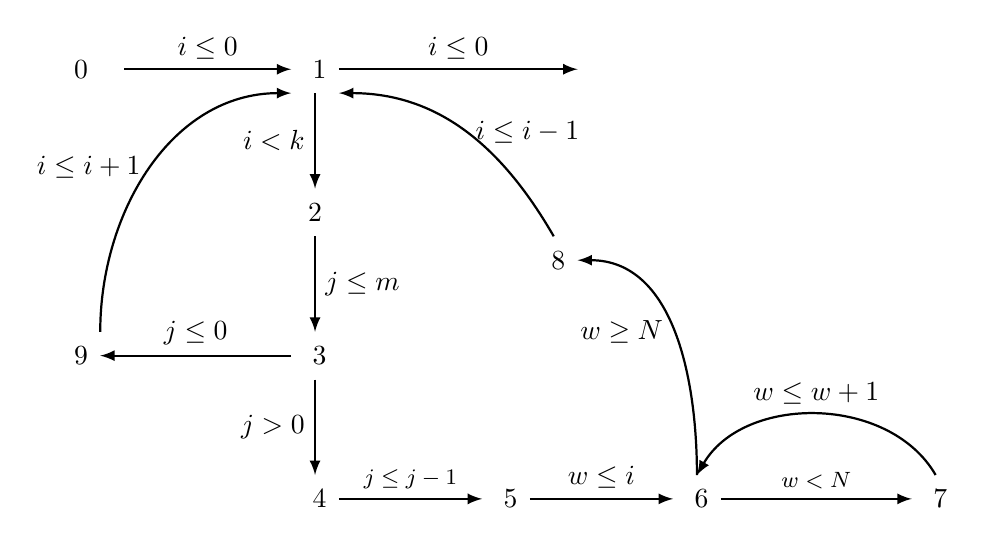
\begin{tikzpicture}[scale=\textwidth/20cm,samples=200]
                \draw[] (-5, 10) circle (0pt) node{{ $0$}};
                \draw[] (0, 10) circle (0pt) node{{ $1$}};
                \draw[] (6, 10) circle (0pt) node {{$\lex$}};
                \draw[] (0, 7) circle (0pt) node{{$2$}};
                \draw[] (0, 4) circle (0pt) node{{ $3$}};
                \draw[] (-5, 4) circle (0pt) node{{ $9$}};
                \draw[] (0, 1) circle (0pt) node{{ $4$}};
                \draw[] (4, 1) circle (0pt) node{{ $5$}};
                \draw[] (8, 1) circle (0pt) node{{ $6$}};
                \draw[] (13, 1) circle (0pt) node{{ $7$}};
                \draw[] (5, 6) circle (0pt) node{{ $8$}};
                % Counter Variables
                %
                % Control Flow Edges:
                \draw[ thick, -latex] (-4, 10)  -- node [above] {$i \leq 0$}(-0.5, 10);
                \draw[ thick, -latex] (0, 9.5)  -- node [left] {$i < k$} (0, 7.5) ;
                \draw[ thick, -latex] (0, 6.5)  -- node [right] {$j \leq m$} (0, 4.5) ;
                \draw[ thick, -latex] (0, 3.5)  -- node [left] {$j > 0$} (0, 1.5) ;
                \draw[ thick, -latex] (-0.5, 4)  -- node [above] {$j \leq 0$} (-4.5, 4) ;
                \draw[ thick, -latex] (-4.5, 4.5)  to  [out=90,in=180]  node [left] {$i \leq i + 1$ }(-0.5, 9.5);
                \draw[ thick, -latex] (0.5, 10)  -- node [above] {$i \leq 0$}  (5.5, 10);
                \draw[ thick, -latex] (0.5, 1)  -- node [above] {{\footnotesize $j \leq j - 1$}}  (3.5, 1);
                \draw[ thick, -latex] (4.5, 1)  -- node [above] {$w \leq i$}  (7.5, 1);
                \draw[ thick, -latex] (8.5, 1)  -- node [above] {{\footnotesize $w < N$}}  (12.5, 1);
                \draw[ thick, -latex] (8, 1.5)  to [out=90,in=0] node [left] {{$w \geq N$}}  (5.5, 6);
                \draw[ thick, -latex] (13, 1.5)  to  [out=120,in=60] node [above] {$w \leq w + 1$}  (8, 1.5);
                \draw[ thick, -latex] (5, 6.5)  to  [out=120,in=0]  node [right] {$i \leq i - 1$ }(0.5, 9.5);
                \end{tikzpicture}
%     \caption{}
%     \end{centering}
%     \end{subfigure}
% \begin{subfigure}{.2\textwidth}    
% \begin{centering}
    {\small
$
    \begin{array}{ll}
        \tpath_0 = (0 \to 1)
        &
        \tpath_4 = (6 \to 8 \to 3)
        \\        
        \tpath_1 = (1 \to 2 \to 3)
        &
        \tpath_5 = (3 \to 9 \to 1)
        \\
        \tpath_2 = (3 \to 4 \to 5 \to 6)
        &
        \tpath_6 = (1 \to \lex)
        \\
        \tpath_3 = (6 \to 7 \to 6)
    \end{array}
$
}
\vspace{-0.2cm}
\caption{}
\end{centering}
\end{subfigure}
% $
%     \begin{array}{l}
%         \rprog_1 = {\rprepeat(\tpath_1; 3: {\rprepeat(\tpath_2; 6 : {\rprepeat(\tpath_3)}; \tpath_4)}; \tpath_5)}
%         \\
%         \rprog_3 = {\rprepeat(\tpath_2; 6 : {\rprepeat(\tpath_3)}; \tpath_4)}
%     \end{array}
% $
$\rprog = \tpath_0; 1: \rprepeat(\tpath_1; 3: {\rprepeat(\tpath_2; 6 : {\rprepeat(\tpath_3)}; \tpath_4)}; \tpath_5);\tpath_6$
\vspace{-0.2cm}
\caption{
    (a) An example of three nested loops with related iterators,
    (b) the abstract transition graph, simple transition paths and loop body.}
    \vspace{-0.8cm}
        \label{fig:threeWhile-overview}
    \end{figure}
